\section{Evaluation}
Evaluation of the system is performed by testing the deployed \ac{io} server and web application with several Android devices which are available.
The functionality of the system is evaluated to determine if trips are correctly divided and data captured is sound.

\begin{table}[H]
\caption{Android devices tested}
\label{tab:android_devices_tested}
\begin{tabular}{llll}
\hline
Android Device      & Price[R]  & Major Android Version & Linear Accelerometer \\ \hline
Huawei P8 Lite 2017 & 2900     & 8                     & Yes                  \\
Samsung Galaxy A01  & 2180     & 10                    & No                   \\
Galaxy A3 Core      & 1400     & 10                    & No                   \\
Huawei Nova 5T      & 7700     & 10                    & Yes                  \\ \hline
\end{tabular}
\end{table}

\subsection{Logging accuracy}
Generally, \ac{gps} accuracy is reasonable, within an approximately 20 meter range.
Occasionally, a rogue data point occurs resulting in a random spike, as shown in figure \ref{fig:random_spike}.
A small adjustment is made to algorithm \ref{algo_agg}, where the proceeding log is also compared with the current log in each iteration of the for loop.
This ensures that two consecutive logs must be greater than the distance threshold, when aggregating nearby data points.
The result of this correction is depicted in figure \ref{fig:random_spike_correct}.

\begin{figure}[H]
\centering
    \subfigure[Random spike]
    {
        \centering
        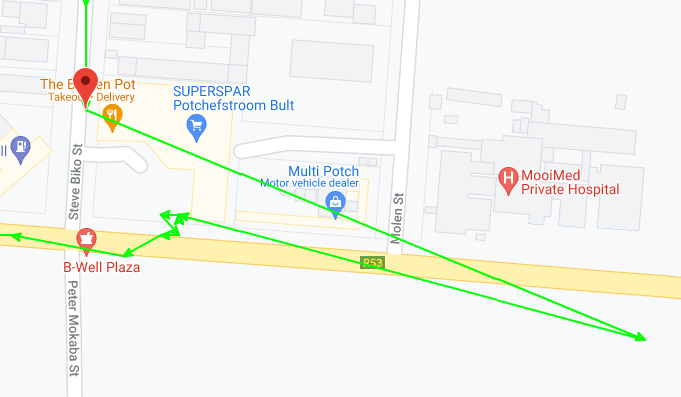
\includegraphics[width=2.5in]{random_spike.png}
        \label{fig:random_spike}
    }
    \subfigure[Correction]
    {
        \centering
        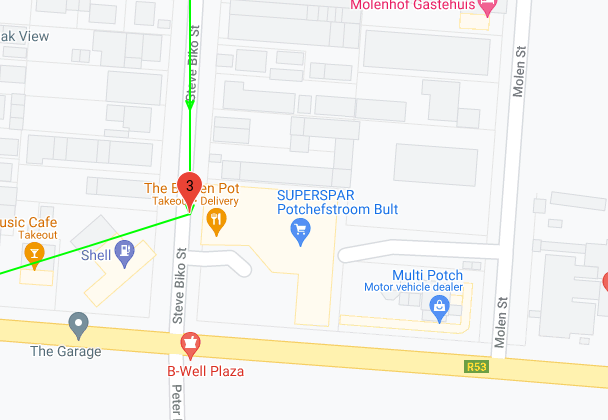
\includegraphics[width=2.5in]{random_spike_correct.png}
        \label{fig:random_spike_correct}
    }
\caption{Location spike correction}
\label{fig:spike_correction}
\end{figure}

\begin{figure}
\centering
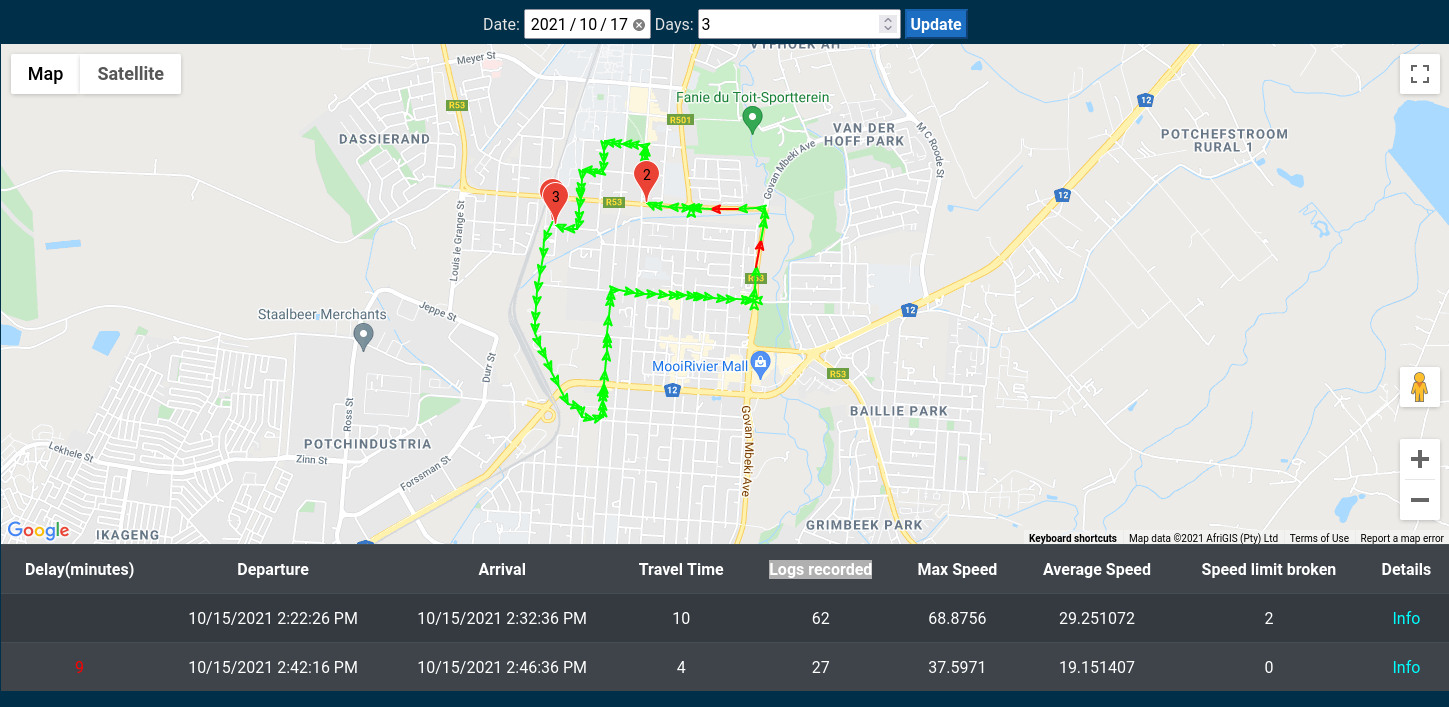
\includegraphics[width=6in]{eval_location.png}
\caption{Location Tracking}
\label{fig:eval_location}
\end{figure}

\begin{figure}
\centering
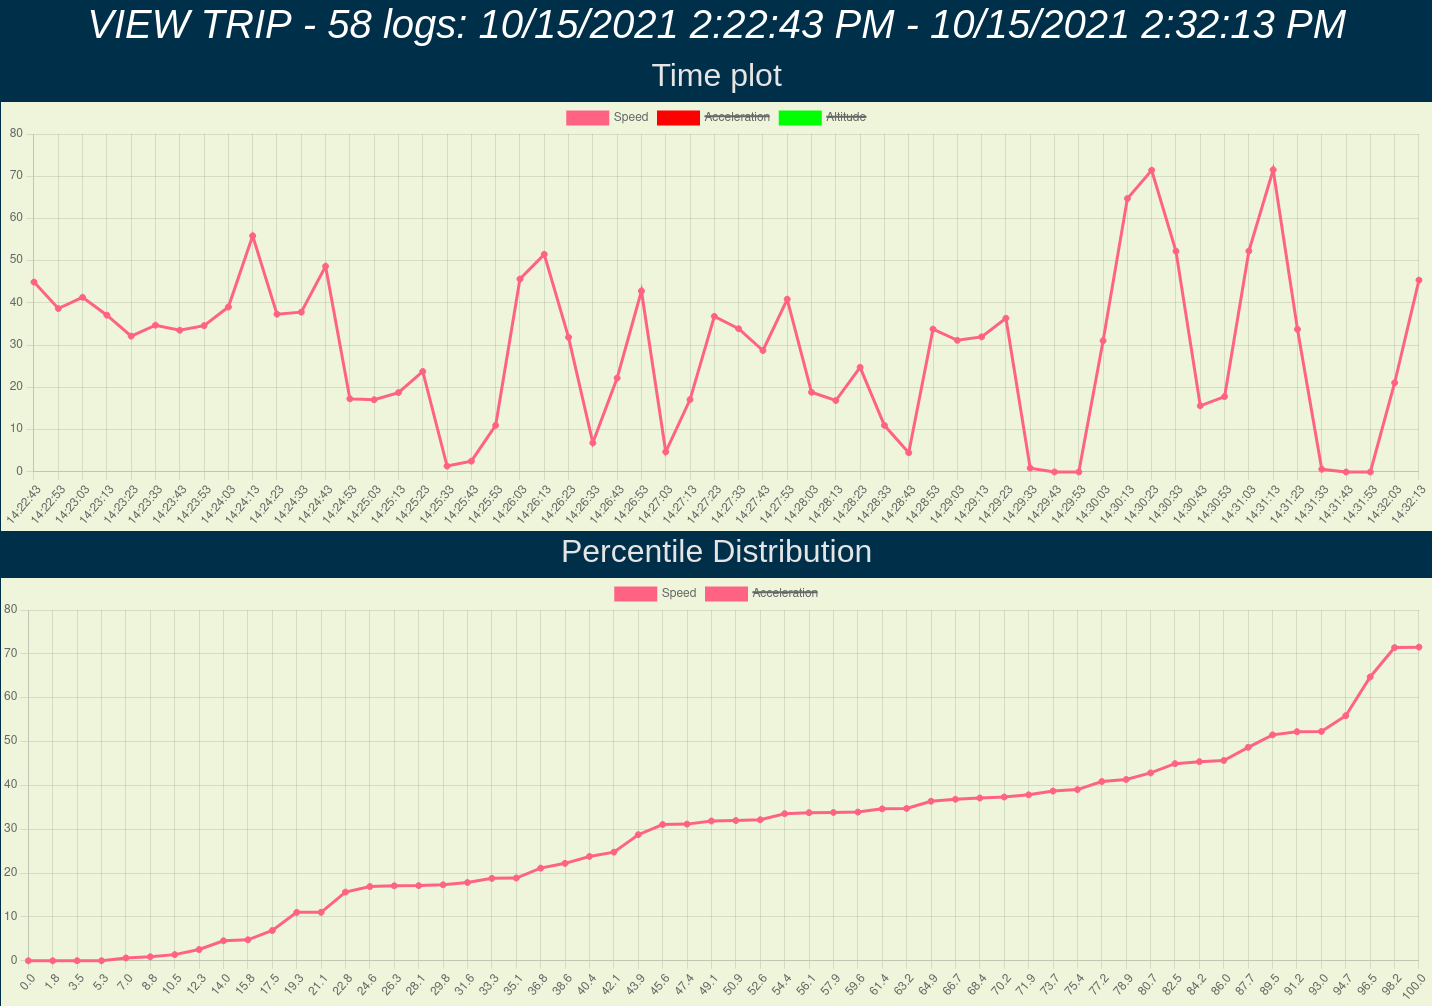
\includegraphics[width=5in]{eval_speed.png}
\caption{Speed Capture}
\label{fig:eval_speed}
\end{figure}

The four devices are taken on the same trip, with the logging interval set to 10 seconds.
The first trip is performed more erratically, with more rapid acceleration and speed.
Afterwards, the return trip is performed in a slower passive manner.

All devices register near-identical arrival and departure times, and sketch the same route on the map, as depicted above in figure \ref{fig:eval_location}.
With the speed limit set to \SI{60}{\kilo\meter\per\hour}, portions of the trip were correctly logged above this speed.
Data captured for all devices indicate similar trends.

Figure \ref{fig:eval_speed} above depicts the time and percentile plots for the speed data collected on the first trip.
This data accurately captures the speeds that were driven.

\begin{figure}[H]
\centering
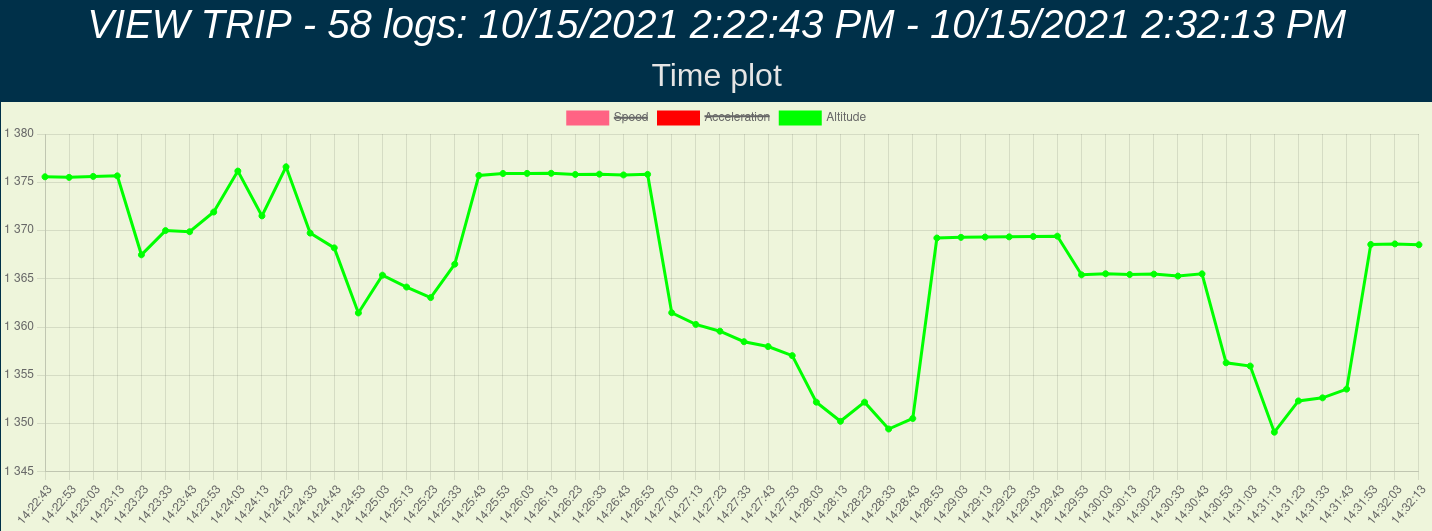
\includegraphics[width=5in]{eval_altitude.png}
\caption{Altitude Data}
\label{fig:eval_altitude}
\end{figure}

Altitude is also captured and displayed in figure \ref{fig:eval_altitude}.
With the quoted altitude for the region at \SI{1340}{ \metre }, the measured altitude values are within error margins.

Figure \ref{fig:accel} below details acceleration data for an erratic trip compared to a passive trip.
The passive trip, in figure \ref{fig:eval_accel_slow} shows a smoother curve with less pronounced spikes. The spread of the logged acceleration stays below \SI{2}{\metre \per \square \second}.
The erratic trip, in figure \ref{fig:eval_accel_fast} indicates more pronounced spikes in acceleration data, and greater acceleration above the 95th percentile.
This acceleration data clearly distinguishes passive driving from erratic driving.

\begin{figure}[H]
\centering
    \subfigure[Erratic]
    {
        \centering
        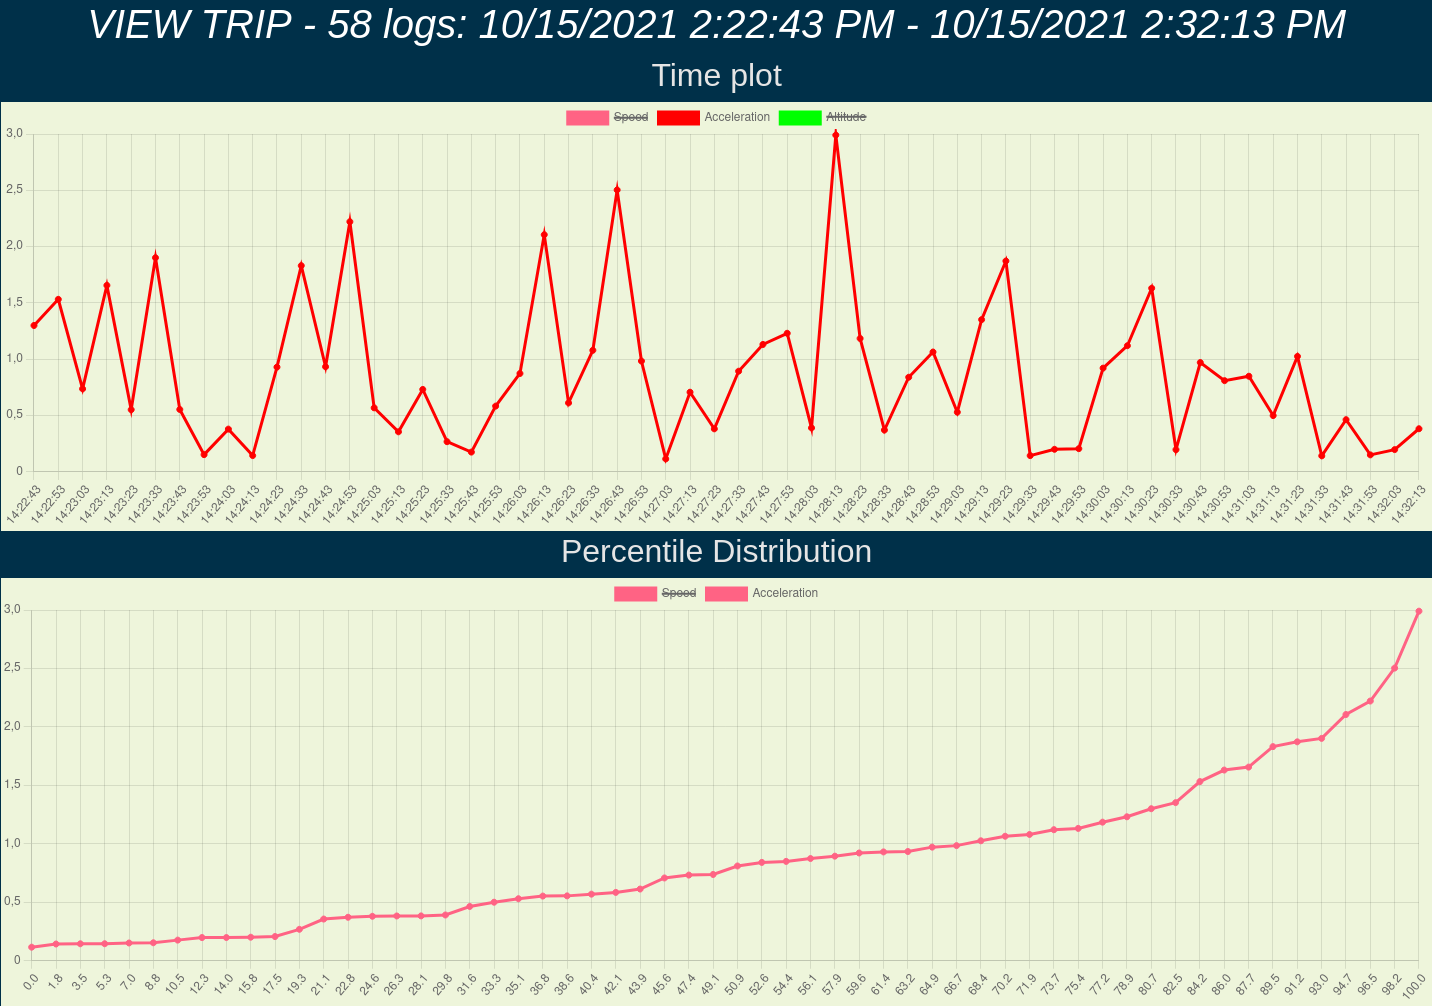
\includegraphics[width=5in]{eval_accel.png}
        \label{fig:eval_accel_fast}
    }
    \subfigure[Passive]
    {
        \centering
        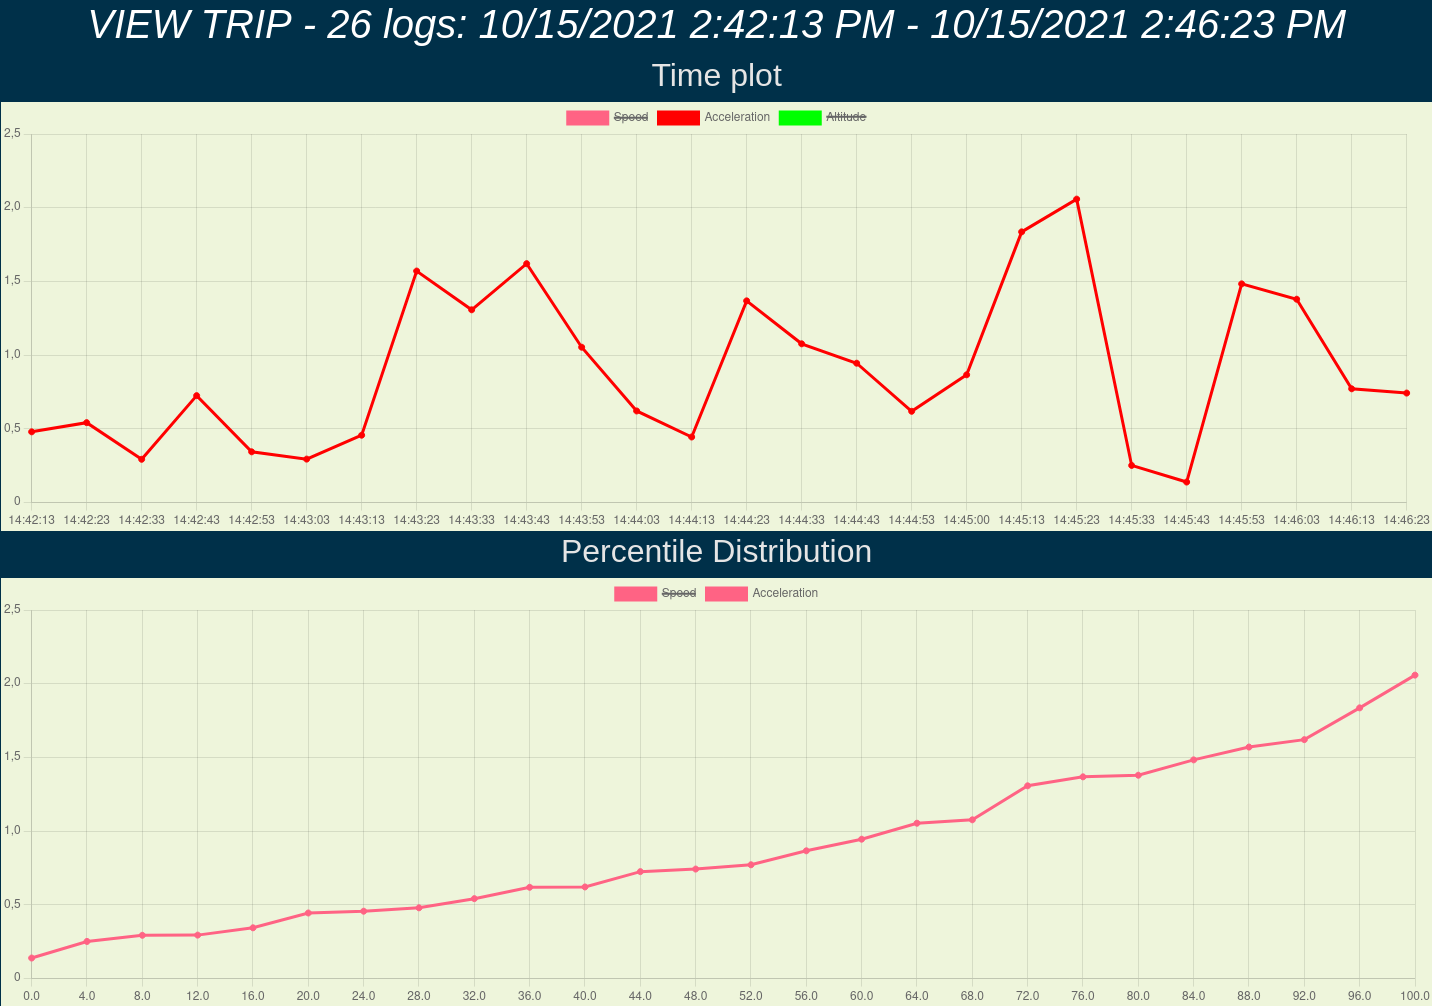
\includegraphics[width=5in]{eval_accel_slow.png}
        \label{fig:eval_accel_slow}
    }
\caption{Acceleration comparison for different driving behavior}
\label{fig:accel}
\end{figure}


\subsection{Android application}
Four Android devices were readily available for testing purposes, which are highlighted in table \ref{tab:android_devices_tested}.

\subsubsection{Application reliability}
Application reliability is tested by ensuring that the tracking service remains active indefinitely.
It is noted that on the Huawei P8 Lite 2017 (running Android 8), the service crashes and stops logging every few hours.
Checking Android debug logs revealed little as to the cause of this crash.

All devices running Android 10 run indefinitely without issue.

\subsubsection{Application Profiling}
The application is profiled in the Android Studio, generating plots for \ac{cpu}, \ac{ram} and network usage as shown in figure \ref{fig:android_profiling}.
\begin{figure}[H]
\centering
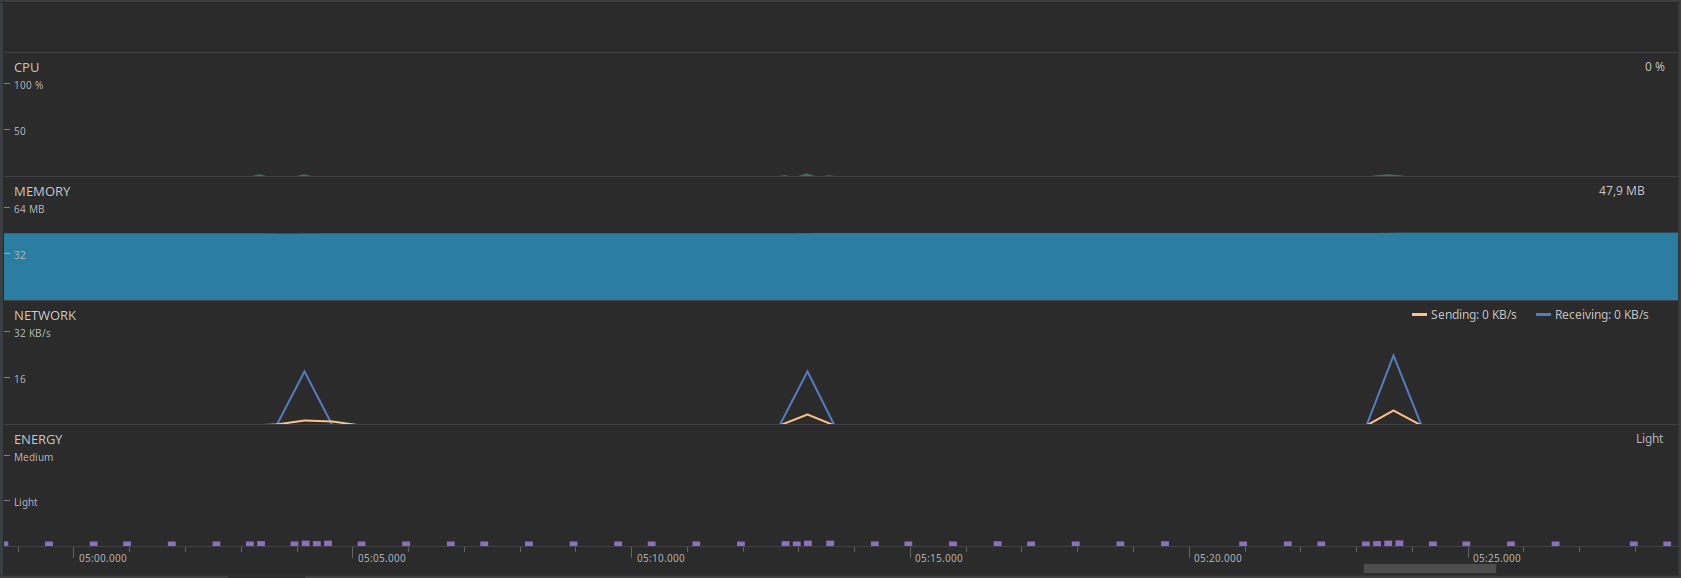
\includegraphics[width=6in]{android_profiling.png}
\caption{Android Profiling}
\label{fig:android_profiling}
\end{figure}
It is noted that the application runs relatively lightly on the system, consuming minimal power and \ac{cpu}.
Typically only 50MB of \ac{ram} is utilized by the application.

\begin{figure}[H]
\centering
    \subfigure[Data Usage]
    {
        \centering
        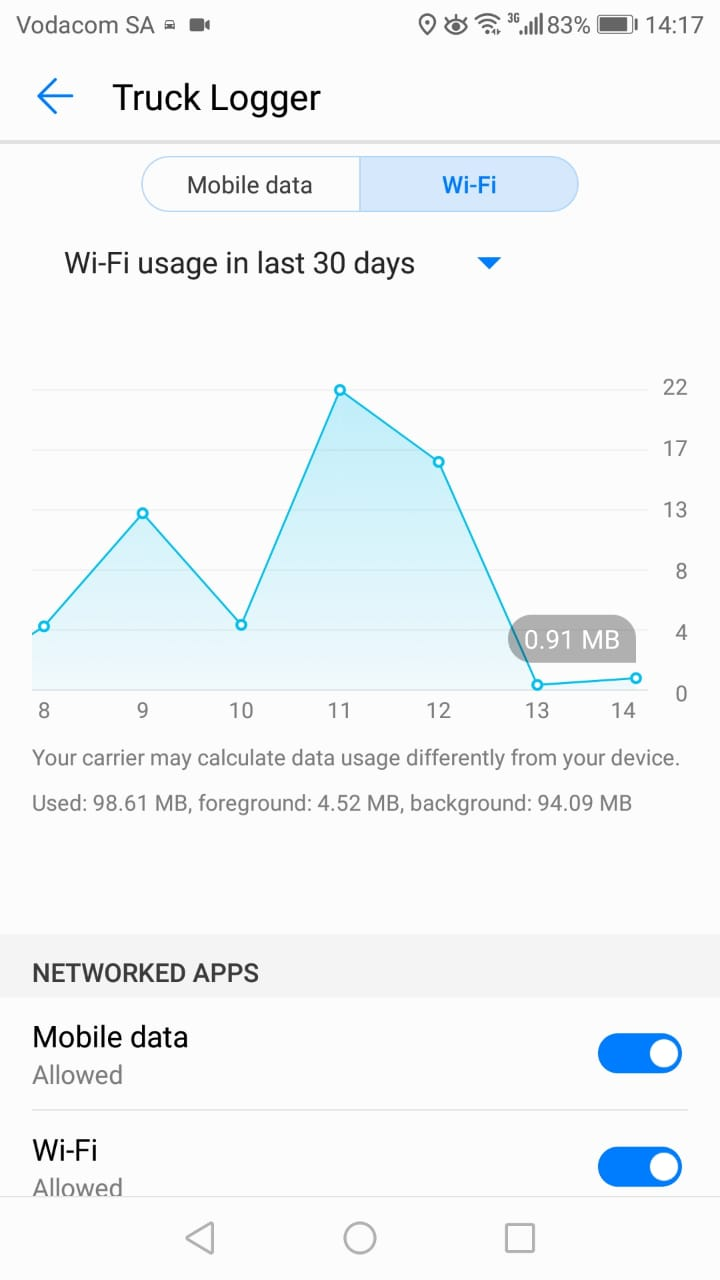
\includegraphics[height=2.5in]{android_data_usage.jpeg}
        \label{fig:android_data_usage}
    }
    \subfigure[Up Time]
    {
        \centering
        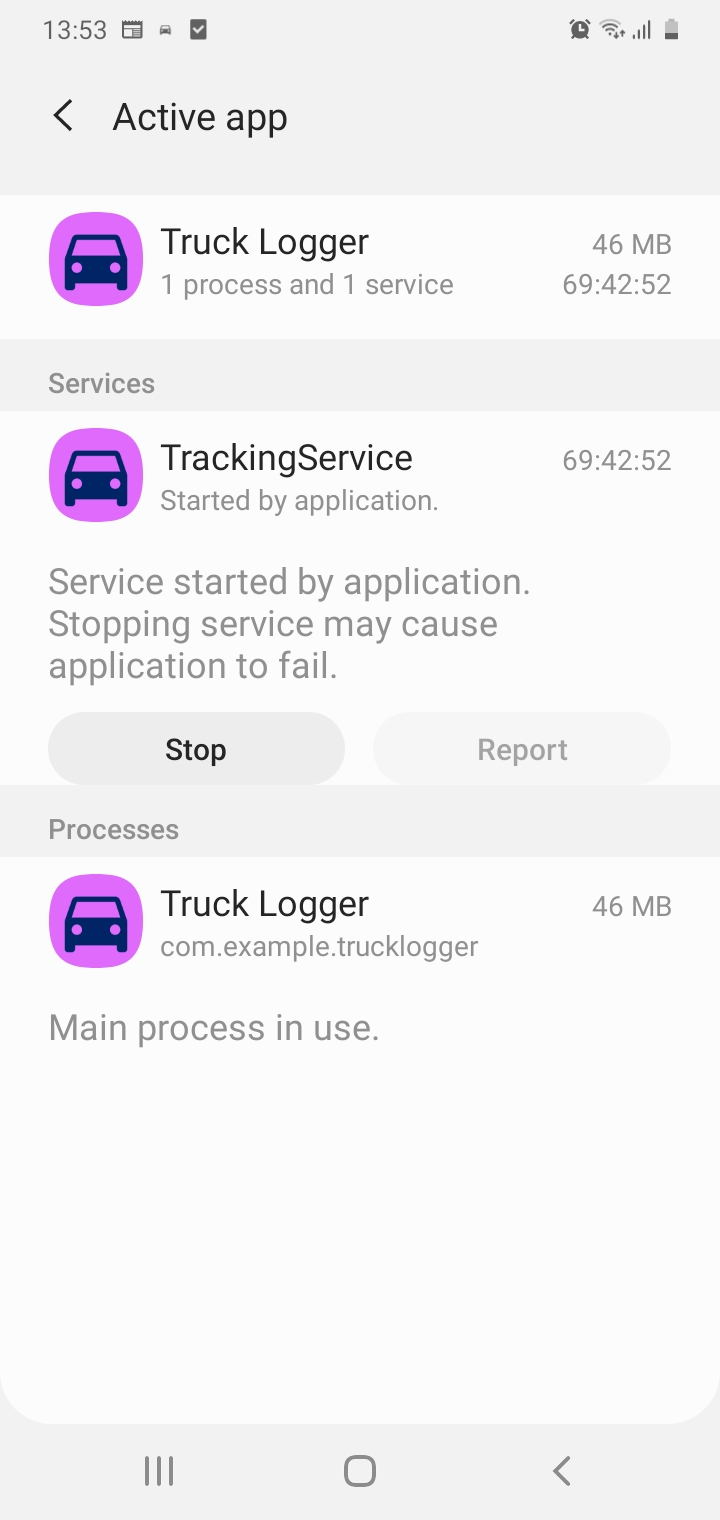
\includegraphics[height=2.5in]{android_app_uptime.jpeg}
        \label{fig:android_app_uptime}
    }
\caption{Android application - up time and data usage}
\label{fig:performance}
\end{figure}

Figure \ref{fig:android_data_usage} details monthly data usage during development on the Huawei P8 Lite 2017, during which the application was logging at a 5 second interval.
In this time, the application consumed approximately 100MB of data.

Figure \ref{fig:android_app_uptime} details the up-time of the application on the Galaxy A3 Core.
The application is seen achieving uninterrupted up-time of approximately 70 hours.

\subsection{\Ac{io} server and web application}
Due to adequate exception handling, both the \ac{io} server and web application remain online indefinitely.
Any exceptions that occur with parsing data are properly handled, without compromising data.

\pagebreak
